\documentclass{beamer} %
%\usetheme{CambridgeUS}
\usepackage[latin1]{inputenc}
%\usefonttheme{professionalfonts}
\beamertemplatenavigationsymbolsempty
\usepackage{times}
\usepackage{tikz}
\usepackage{amsmath}
\usepackage{verbatim}
\usetikzlibrary{positioning,shapes,shadows,arrows}

%style
\tikzstyle{every picture}+=[remember picture]
\definecolor{azul}{RGB}{29,186,222}
\definecolor{morado}{RGB}{161,29,222}
\definecolor{marron}{RGB}{223,66,30}
\definecolor{verde}{RGB}{90,222,29}

%node style
\tikzstyle{frame}=[rectangle, rounded corners, text centered, anchor=north, text width=2.5cm, text=black, draw=black!50!azul!50, top color=white, bottom color=azul]
\tikzstyle{program}=[morado]
\tikzstyle{label}=[marron]

%arrow styles
\tikzstyle{fixed}=[->, black!50, thick]
\tikzstyle{estimation}=[->, morado, thick, dashed]
\tikzstyle{difference}=[->, marron, thick, dotted]
\tikzstyle{source}=[->, verde, thick]
\tikzstyle{skip loop}=[to path={-- ++(0,#1) -| {\tikztotarget}}]


%metadata
\title{Integration of multiple localization systems into TF}
\author{Pablo Urcola \\ \texttt{urcola@unizar.es}}
\institute{Robotics, Perception and Real Time Group\\ Universidad de Zaragoza, Spain}
\date{ROS Community Workshop\\ 2015 European Robotics Forum}

\begin{document}

\begin{frame}
\titlepage
\end{frame}

\begin{frame}
%\frametitle{TF tree}
\vspace{4cm}
%\begin{figure}[*ht]
\begin{center}
\begin{tikzpicture}[node distance=1.0cm, auto, overlay]
%nodes
	\node<1-> [frame]                                (robot) {robot};
	\node<2-> [frame, above=of robot]                (odom) {odom};
	\node<3-> [frame, above=of odom]                 (map) {map};
	\node<4-> [program, right=of odom] (amcl) {AMCL};
	\node<5-> [label, above=of odom, xshift=-1.0cm, yshift=-0.75cm] (mapcorrection) {Correction};
	\node<6-> [frame, above=of map]                  (gps) {gps};
	\node<7-> [program, left=of odom, xshift=-0.9cm]  (ekf) {EKF};
	\node<7-> [frame, below=of robot]                (antenna) {antenna};	
	\node<8,9> [label, above=of map, xshift=-1.0cm, yshift=-0.75cm] (gpscorrection) {Correction};
	\node<10> [program, right=of gps, yshift=-0.5cm] (manager) {Manager};

%edges		
	\path<2-> (odom) edge [estimation, out=270, in=90] node[auto, swap] {Odometry} (robot);
	\path<4-> (map) edge [estimation, out=0, in=0] (robot);
	\path<5-> (map) edge [difference, out=270, in=90] (odom);
	\path<5-9> (amcl) edge [source, out=180, in=0] (mapcorrection);
	\path<7-> (robot) edge [fixed, out=270, in=90] node[auto] {Fixed} (antenna);
	\path<7-> (gps) edge [estimation, out=180, in=180] (antenna);
	\path<8-> (gps) edge [difference, out=270, in=90] (map);
	\path<8,9> (ekf) edge [source, out=0, in=180] (gpscorrection);
	%\path<8,9>   (amcl)  edge [source, out=180, in=0]       										 (gpscorrection);	
	\path<10> (gps) edge [fixed, out=270, in=90] node[auto] {Fixed} (map);
	\path<10> -- (4,4) -- (ekf) edge [source, out=100, in=130] (manager);
	\path<10> (amcl) edge [source, out=0, in=0] (manager);
	\path<10> (manager) edge [source, out=270, in=0] (mapcorrection);
\end{tikzpicture}
\end{center}
%\end{figure}
\vspace{2cm}
\uncover<9>{Problem: Where is the robot in the map frame?}

\uncover<10>{AMCL and EKF do not directly manage the correction}
\end{frame}

\begin{frame}
%\frametitle{Conclusions}
\begin{itemize}
	\item Multiple estimation of robot position cannot be directly introduced into TF
	\item The map-odom correction technique is not scalable as it does not provide the best estimation in every frame
	\item Only one correction point
	\item An external manager requires the ability to disable the tf publishers
\end{itemize}
\end{frame}

\end{document}
